\chapter{Ice Reservoirs}

\cleanchapterquote{Glaciers are the secret of life in these otherwise lifeless deserts. But now, they are
melting away at an alarming rate.}{Sonam Wangchuk}{(Ramon Magsaysay awardee, Inventor of ice stupas)}


\section{Introduction}

Mountains contribute disproportionally to global water resources compared with their geographical extent and are
therefore often described as natural water towers \citep{immerzeelImportanceVulnerabilityWorld2020}. Because of
their buffering capacity, for instance by supplying glacial melt water during the hot and dry season, they
provide a relatively constant water supply to downstream areas. Worldwide, the vast majority of glaciers are
losing mass \citep{zempGlobalGlacierMass2019a}, snow melt dynamics are being perturbed
\citep{mukhopadhyayReevaluationSnowmeltGlacial2015, hammondGlobalSnowZone2018}, and precipitation and
evapotranspiration patterns are shifting, all leading to future vulnerability of mountain water availability
\citep{lutzConsistentIncreaseHigh2014}. These issues are particularly pronounced in arid and semiarid regions,
where it is estimated that between 50 \% and 90 \% of freshwater resources originate from mountain catchments
\citep{mukhopadhyayReevaluationSnowmeltGlacial2015, messerliMountainsWorldVulnerable2004}. There is high
confidence that these changes are largely negatively impacting agriculture across many different mountainous
regions \citep{ipccCrossChapterPaperMountains2022}.  

Since water supply and demand are linked at the river basin scale, we classify basins as \ac{WTUs} following
\citet{immerzeelImportanceVulnerabilityWorld2020}. Globally there are 78 \ac{WTUs}, which are home to more than
250 million people. Among these, the three most important water towers lie in Central Asia due to their
relatively high glacial water supply and irrigation water demand (Fig. \ref{fig:WTUs_AIRs}). As a consequence, mountain communities in these regions have
developed several innovation water storage solutions and farming practices to cope with climate change induced
water stress \citep{labbalTraditionalOasesLadakh2000, nusserIrrigationDevelopmentUpper2012, kreutzmannScarcityOpulenceWater2011, pandeyRockGlacierOasis2022,
ochoa-tocachiPotentialContributionsPreInca2019, monge-salazarEcohydrologyEcosystemServices2022}.

\begin{figure}[htb]
\centering
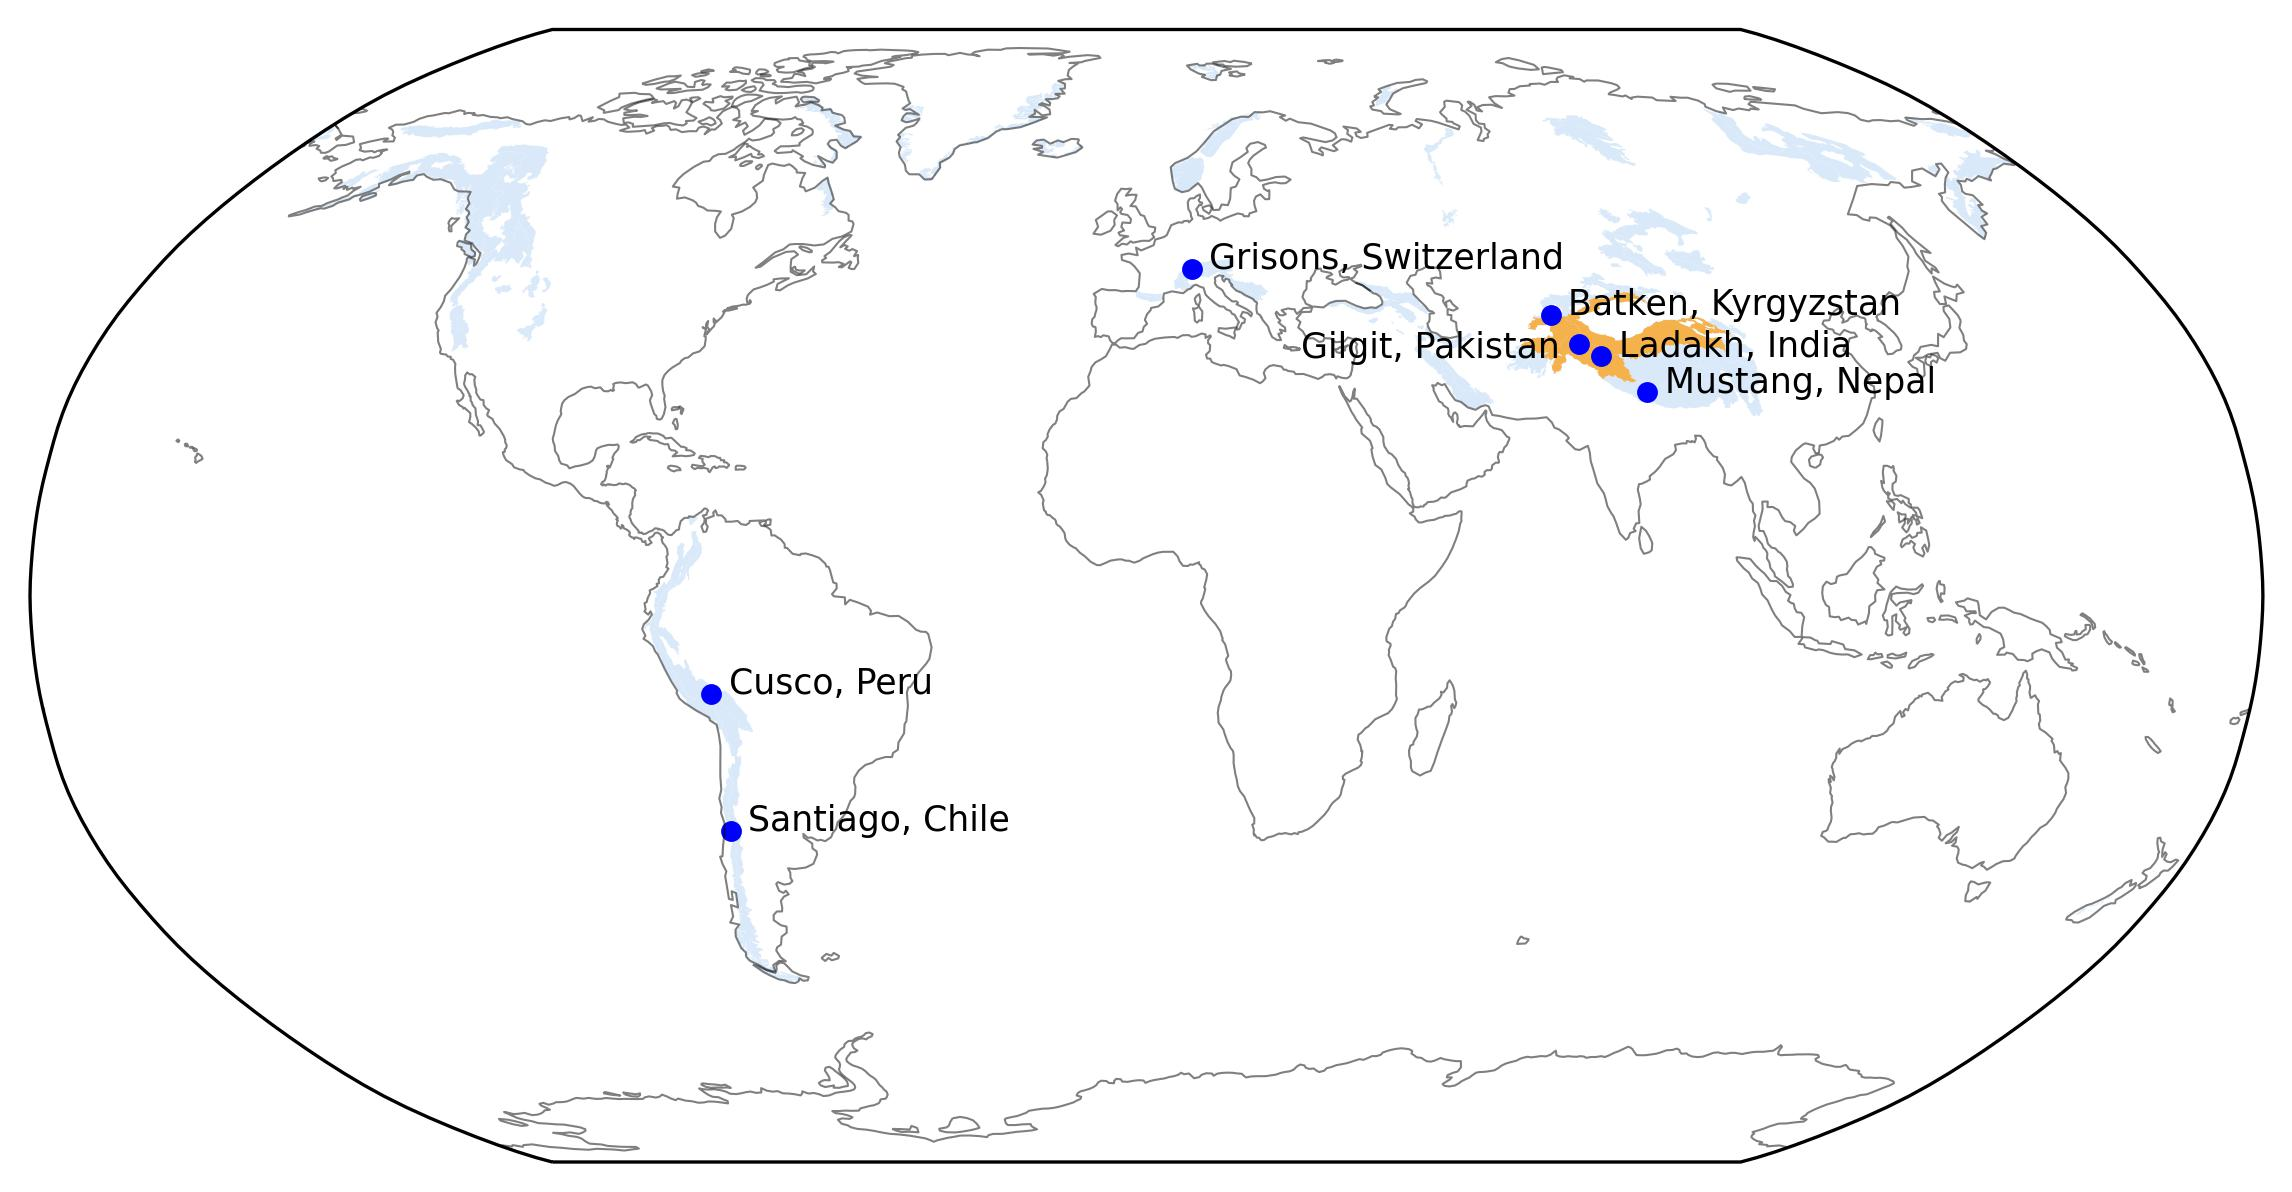
\includegraphics[width=\textwidth]{figs/WTUs_AIRs.jpg}

\caption{ Among all the water tower units (light blue), the most important ones (orange) are also where most of
  the AIR construction sites  are located (dark blue). Adapted from
\cite{immerzeelImportanceVulnerabilityWorld2020}.} 

\label{fig:WTUs_AIRs} 
\end{figure}

Especially in the upper Indus basin, there is a long tradition of building \ac{AIRs} with records dating back to
more than 50 years \citep{nusserSociohydrologyArtificialGlaciers2019}. \ac{AIRs} capture water in the autumn and
winter, allowing it to freeze, and hold it until spring, when it melts and flows down to the fields
\citep{ipccChapterHighMountain2019, vinceGlacierMan2009, clouseLadakhArtificialGlaciers2017,
nusserSociohydrologyArtificialGlaciers2019}. In this way, they retain a previously unused portion of the annual
flow and facilitate its use supplementing the decreased flow during the following spring (Fig.
\ref{fig:irrigation_cycles}). Over the past decade, several \ac{AIRs} have been built to supplement the
irrigation water supply of mountain villages in India \citep{wangchukIceStupaCompetition2020,
palmerStoringFrozenWater2022, aggarwalAdaptationClimateChange2021}, Pakistan
\citep{awazproductionIceStupaArtificial2022}, Kyrgyzstan \citep{bbcnewsBrightArtificialGlacier2020}, Nepal, and
Chile \citep{reutersConservationistsChileAim2021}. In total, more than 500 farmers have constructed AIRs across
30 villages in the Alps, Andes and Hindu Kush Himalayas (Fig. \ref{fig:WTUs_AIRs}). 

\begin{figure}[htb] \centering 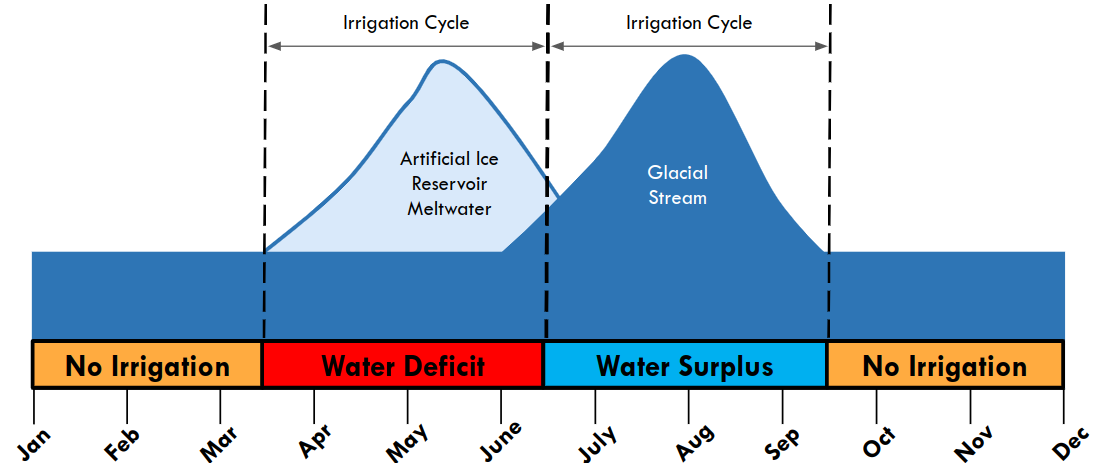
\includegraphics[width=\textwidth]{figs/irrigation_cycles.png}
\caption{Seasonal variation in the availability of irrigation water in Ladakh, India. The graph highlights the
crucial role of \ac{AIRs} in bridging the gap in water availability. Adapted from
\cite{nusserLocalKnowledgeGlobal2016}.} \label{fig:irrigation_cycles} \end{figure}


Despite this widespread adoption, only a few publications examine the role of \ac{AIRs} in the water resource
management of these regions. Notably, none of these prior reports have investigated \ac{AIRs} outside Ladakh.
Moreover, the available estimates of water storage capacity of \ac{AIRs} in Ladakh vary widely
\citep{norphelSnowWaterHarvesting2015, baglaArtificialGlaciersHelp1998}.

Quantifying the water storage capacity of \ac{AIRs} is not straightforward since the processes by which
\ac{AIRs} are formed are complex. These processes are controlled by local topography, meteorology and the
construction strategies used. Modelling approaches to quantifying these processes exist on glacier surfaces but
they are not readily applicable for \ac{AIRs} due to their limited size, and comparatively more variable surface
area. Therefore, conventional modelling approaches used in glaciology need to be adapted in order to capture the
spatio-temporal scale of AIR surface processes. Furthermore, these modelling approaches need to be validated and
calibrated with comprehensive data from field measurements. 

A spirit of improvisation guides the construction of \ac{AIRs} \citep{clouseLadakhArtificialGlaciers2017}.
Depending on the local topography and on how water is supplied, \ac{AIRs} can form as flat sheets or vertical
cones and are, therefore, referred as ice terraces and ice stupas respectively (Fig. \ref{fig:AIRforms}). This
has resulted in \ac{AIRs} exhibiting significant volume variations despite experiencing similar
meteorological conditions. For example, in Ladakh, India, ice terraces have attained volumes up to 30 times
larger than ice stupas \citep{nusserSociohydrologyArtificialGlaciers2019}. However, the processes driving these
differences can only be understood if the complete design methodology behind each construction is available.

\begin{figure}[t]
\centering
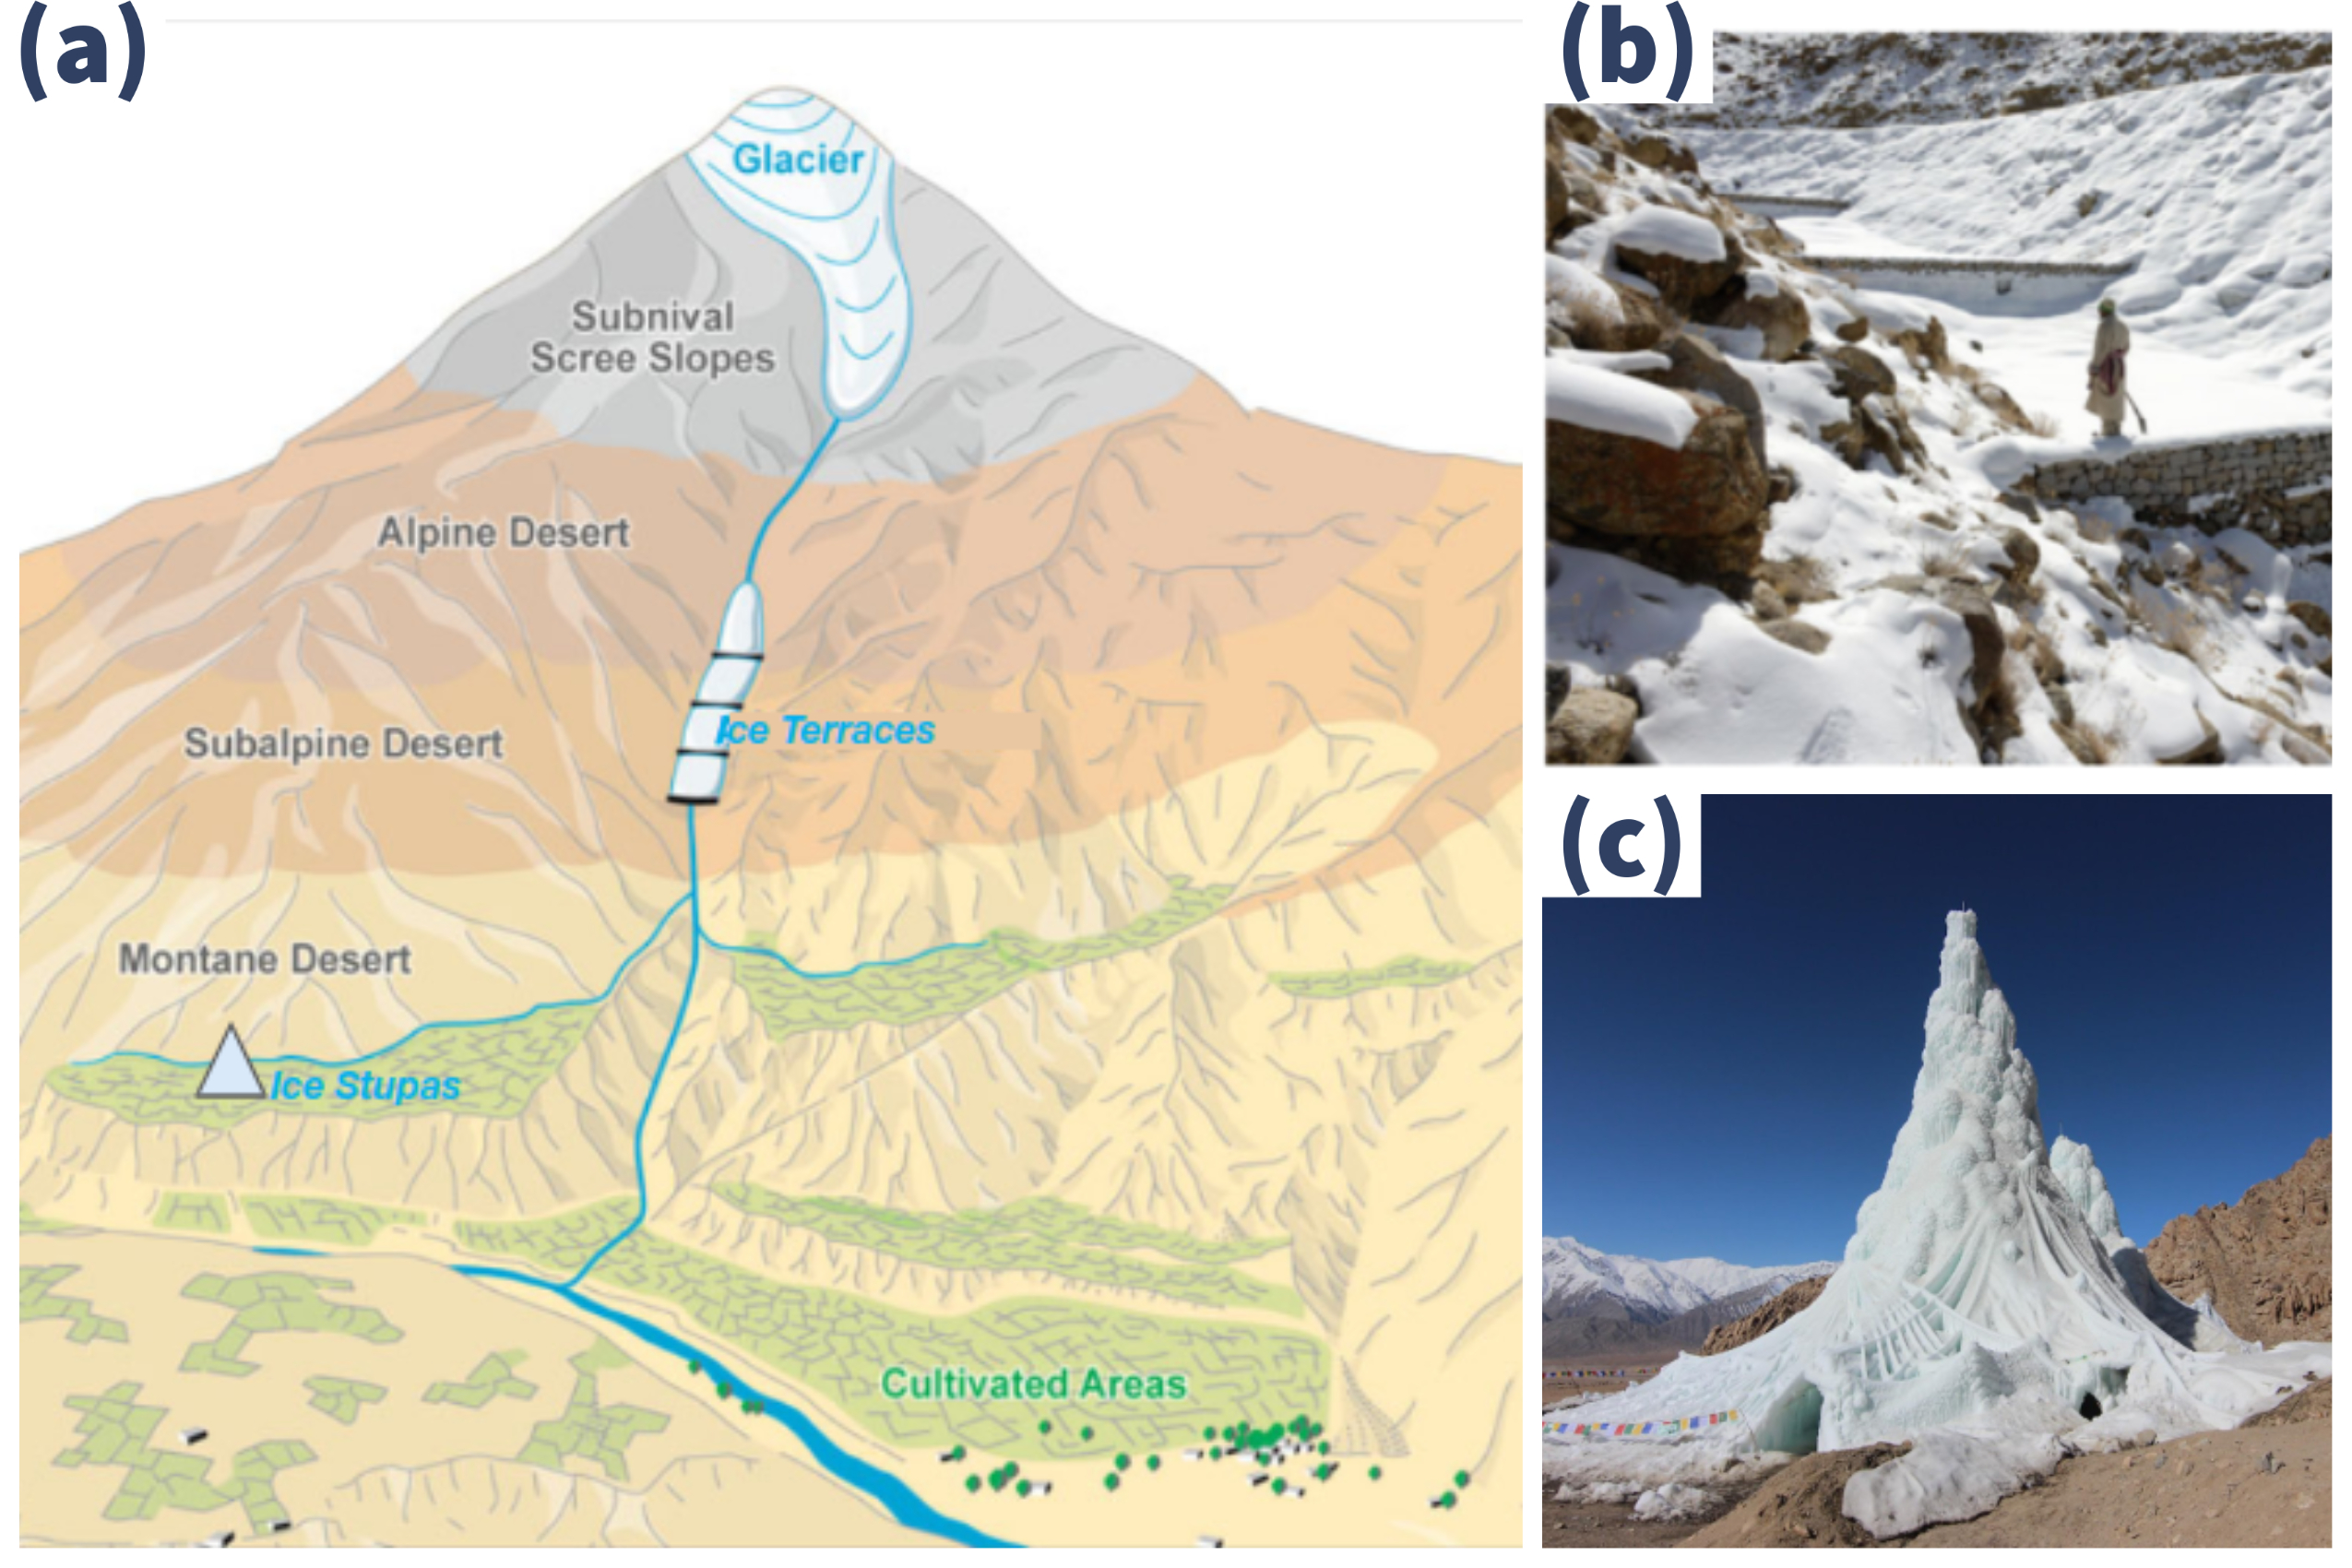
\includegraphics[width=\textwidth]{figs/AIR_forms.jpg}

\caption{ (a) Schematic overview of the position of artificial ice reservoirs. These constructions are located at
  altitudes between the glaciers and the irrigation networks in the cultivated areas. (b) Ice terraces at 3900
  $m$ \{a.s.l.}, located above the village of Nang, Ladakh. The cascade is composed of a series of loose masonry walls
  ranging in height from 2 to 3 $m$, which help to freeze water for storage. (c) Ice stupas at 3600 m, located
above the village of Phyang, Ladakh. They are made using fountain systems. Adapted from \cite{nusserLocalKnowledgeGlobal2016}. }

\label{fig:AIRforms}
\end{figure}

This thesis aims to fulfill both these requirements by providing a new set of AIR-specific volume and area
measurements via drone flights, along with meteorological data during the construction period. All these
datasets were generated through construction strategies that used fountain systems. These systems are quantified
via in-situ observations of the fountain characteristics and discharge rate measurements. First, a
one-dimensional AIR model is formulated in order to calibrate and validate it with the procured AIR datasets.
Then the model is used as a tool to propose a construction strategy that can produce \ac{AIRs} efficiently and
effortlessly. We acknowledge that the farming communities building these structures since the mid-1800s are the
custodians of substantial additional knowledge.


\section{Nomenclature and Classification}

The term "artificial glacier" is more commonly used by local farmers to refer to \ac{AIRs}
\citep{norphelArtificialGlacierHigh2009}. However, many believe this terminology can be misleading
\citep{nusserSociohydrologyArtificialGlaciers2019}. By definition, all glaciers, including the smallest ones,
are bodies of sedimentary ice, which were built by progressive snow compaction and firnification and flow
downhill under the influence of gravity \citep{benndouglasGlaciersGlaciation2014}. Hence, because of their
genesis and composition, \ac{AIRs} differ from glaciers. Man-made ice structures typically have a lifetime in
the order of months and a size million times smaller than typical glaciers. We use the terminology \ac{AIRs} to
distinguish the man-made ice structures described in this thesis from the natural ones. 

However, when classified in terms of size and survival duration, \ac{AIRs} exhibit similar characteristics to
very small glaciers. The glossary of glacier mass balance and related terms by
\citet{cogleyGlossaryGlacierMass2010} defines very small glaciers or glacierets as follows:

\begin{thesis_quotation}
  A very small glacier, typically less than 0.25 $km^2$ in extent, with no marked flow pattern
  visible at the surface. To qualify as a glacieret, an ice body must persist for at least two consecutive
  years. Glacierets can be of any shape, and usually occupy sheltered parts of the landscape. Windborne snow and
  avalanches can be dominant contributors to the accumulation of glacierets.
\end{thesis_quotation}

This rather broad definition of glacierets or very small glaciers may be best suited to describe AIRs, since
they have been measured with areas as high as 0.15 $km^2$ \citep{nusserSociohydrologyArtificialGlaciers2019} and
observed to last beyond a year.

As noted above, AIR's construction strategies are usually inspired by a spirit of improvisation which challenges
their classification. However, it has been found that construction strategies using fountain systems form
conical \ac{AIRs}, while those that don't form flat sheets of ice. \ac{AIRs} using fountain systems are called
"ice stupas" and those without are called "ice terraces" as this terminology denotes the resulting shape of the
respective \ac{AIRs} appropriately.

\section{Objectives}

This study employs an integrated approach, which includes field measurements and modelling, to answer the
following research questions: 

\begin{enumerate}

\item What is the influence of construction location and fountain characteristics on ice stupa volume evolution? 

\item How can ice stupa fountain systems be engineered to reduce their water losses and maintenance efforts?

\end{enumerate}

An energy and mass balance model for \ac{AIRs} was designed to answer the first research question (paper I and
III). Since in-situ measurements were required to run this model, we executed a measurement campaign in
Switzerland and India during the past 4 winters (2018/19, 2019/20, 2020/21, 2021/22). These data sets provided
the necessary input, calibration and validation data to model the evolution of \ac{AIRs} and study their
sensitivity to meteorological conditions and fountain characteristics. 

We also developed new construction strategies to answer the second research question. These strategies used the
discharge rate of the fountains regulated by an automation system, which was controled through the AIR
model. Their advantages over traditional construction strategies are quantified in paper II.

\section{Structure}

Chapter 1 introduces the motivation of this work and provides a summary of the state of knowledge about \ac{AIRs}
prior to this thesis. Chapter 2 describes the origins of this technology as a religious practice. Chapter 3
gives an overview about the study sites and introduces the different field techniques applied. The engineering
design of AIR technologies are showcased in Chapter 4 along with suggestions for their improvement. The observed
spatio-temporal variations in AIR volume evolution are presented in Chapter 5 along with suggestions for
choosing future construction locations. Chapter 6 concludes the thesis with a synthesis and some recommendations
for future work. Chapter 7 lays out the peer-reviewed work supporting the conclusions of this thesis.

% There is high confidence that these changes are largely negatively impacting
% agriculture across many different mountainous regions \citep{IPCC}. 

% Global climate change is accelerating glacial ablation in many mountain regions of the world, generating
% concerns about the impact on local and regional water resources \citep{}. 
% Sources of freshwater from mountains, such as rainfall, snow and glacier melt, and groundwater are strongly
% affected by climate change, leading to important changes in water supply in terms of quantity and timing (e.g.
% shifts and changes in seasonality).


% Irrigation networks in arid mountain regions are completely dependent on the timely availability of meltwater
% from glaciers, snow and permafrost
% \citep{immerzeelImportanceVulnerabilityWorld2020,farhanHydrologicalRegimesConjunction2015,tveitenGlacierGrowingLocal2007}.
% With the accelerated decline of glaciers due to climate change \citep{nusserLocalKnowledgeGlobal2016}, these
% regions are experiencing acute water scarcity \citep{norphelSnowWaterHarvesting2015,
% mukhopadhyayReevaluationSnowmeltGlacial2015}. Further, the unreliability and the foreseen decrease of seasonal
% snow cover \citep{chevuturiClimateChangeLeh2018} affects the cryosphere's ability to store water, especially in
% spring.

% More than 700 million people live in mountain areas, of these, around 300 million are vulnerable to food
% insecurity \citep{messerliMountainsWorldVulnerable2004}.

% Especially in the cold-arid Trans-Himalayan region of Ladakh, meltwater supply from the cryosphere is of utmost
% importance for irrigated agriculture in spring and summer, when water demand is highest
% \citep{nusserCryosphereFedIrrigationNetworks2019}. Due to the short growing period, central Ladakh is a
% single-cropping area with barley and wheat as important staples, complemented by vegetables, pulses, and oil
% seeds \citep{nusserSociohydrologyArtificialGlaciers2019}. Depending on the altitude, irrigation with complete
% flooding of fields (approximately 2-5 cm water column) starts between March and April prior to the melting of
% high-altitude glaciers. This results in increased demand during a period of reduced supply at the onset of the
% agricultural season.

% To cope with this recurrent water scarcity, villagers have developed two types of \ac{AIRs}: ice stupas
% and ice terraces (Fig. \ref{fig:AIRforms}). Both the ice reservoirs capture water in the autumn and winter,
% allowing it to freeze, and hold it until spring, when it melts and flows down to the fields
% \citep{ipccChapterHighMountain2019, vinceGlacierMan2009, clouseLadakhArtificialGlaciers2017,
% nusserSociohydrologyArtificialGlaciers2019}. In this way, they retain a previously unused portion of the annual
% flow and facilitate its use to supplement the decreased flow during the following spring (Fig.
% \ref{fig:irrigation_cycles}).

% There is a long tradition of developing ice harvesting structures in the upper Indus Basin, in both Ladakh,
% northern India \citep{labbalTraditionalOasesLadakh2000, nusserIrrigationDevelopmentUpper2012} and various
% locations in northern Pakistan \citep{kreutzmannScarcityOpulenceWater2011}. Villagers here have developed two
% types of \ac{AIRs}: ice stupas and ice terraces (Fig. \ref{fig:AIRforms}). Both the ice reservoirs capture water
% in the autumn and winter, allowing it to freeze, and hold it until spring, when it melts and flows down to the
% fields \citep{ipccChapterHighMountain2019, vinceGlacierMan2009, clouseLadakhArtificialGlaciers2017,
% nusserSociohydrologyArtificialGlaciers2019}. In this way, they retain a previously unused portion of the annual
% flow and facilitate its use to supplement the decreased flow during the following spring (Fig.
% \ref{fig:irrigation_cycles}).

% According to oral history and Corona imagery from 1969, the first ice terraces are older than 50 years. Over the
% past decade, several ice stupas have been built to supplement the irrigation water supply of mountain villages
% in India \citep{wangchukIceStupaCompetition2020, palmerStoringFrozenWater2022,
% aggarwalAdaptationClimateChange2021}, Pakistan \citep{awazproductionIceStupaArtificial2022}, Kyrgyzstan
% \citep{bbcnewsBrightArtificialGlacier2020}, Nepal, and Chile \citep{reutersConservationistsChileAim2021}. In
% total, more than 500 farmers have constructed AIRs across 30 villages in the Alps, Andes and Hindu Kush
% Himalayas (Fig. \ref{fig:WTUs_AIRs}). 
